\documentclass[12pt]{article}

\usepackage[utf8]{inputenc}%encodage des caractères    
                         
\usepackage[T1]{fontenc}%encodage de la police    
                              
\usepackage[french]{babel}%langue française

\usepackage{listings}
\frenchbsetup{StandardLists=true} % à inclure si on utilise \usepackage[french]{babel}

\usepackage{enumitem}

\usepackage[linesnumbered,ruled,french,onelanguage]{algorithm2e}
\usepackage{listings}
	
\usepackage{color}

\usepackage{hyperref}
\usepackage{amsmath}

% Pour l'inclusion des diagrammes UML                                           
\usepackage{graphicx}
\newcommand{\umlscale}{0.4}

% Écriture des noms de classes, etc.                                            
\newcommand{\packagename}[1]{\texttt{#1}}
\newcommand{\classname}[1]{\texttt{#1}}
\newcommand{\methodname}[1]{\texttt{#1}}
\newcommand{\HRule}{\rule{\linewidth}{0.5mm}}

%%%% un bug dans la version française de algorithm2e : pas de traduction de output sans les lignes ci-dessous
\makeatletter 
\g@addto@macro{\@algocf@init}{\SetKwInput{KwOut}{Sortie}} 
\makeatother
%%%%%



\begin{document}

%Page de garde
\begin{titlepage}
	%haut de la page
	\begin{center}
		
\includegraphics[scale=0.2]{Images/logos-Marianne-UNICAEN-scaled.jpg}\\[1.5cm]

		%type de document : rapport
		\textsc{\Large Rapport de Conception Logicielle}\\[1.5cm]

		%Nom du projet
		\HRule \\[0.4cm]
		{
		\LARGE \bfseries A NEW VERSION OF CORE WAR \\[0.2cm]
		}
		\HRule \\[0.5cm]
	\end{center}

	%Equipe Developpement
	\begin{minipage}[c]{0.5\linewidth}
		%Membres du groupes
		\begin{flushleft}
			\underline{Equipe de développement}: \\[0.5cm]
			DOUMBOUYA Sékou\\[0.2cm]
			KITSOUKOU Manne Emile\\[0.2cm]
			OROU-GUIDOU Amirath Fara\\[0.5cm]
			%Info sur la formation
			\underline{Parcours} : Licence 2 Informatique\\[0.2cm]
			\underline{Groupe} : 2B\\
		\end{flushleft}
	\end{minipage}

	%Superviseurs
	\begin{minipage}[c]{\linewidth}
		\begin{flushright}
			\underline{Sous la supervison} :\\[0.5cm]
			BOURDACHE Nadjet \\[0.2cm]
			LECOQ Romain
		\end{flushright}
	\end{minipage}\\[0.7cm]

	%bas de la page de garde
	\center Avril 2022
\end{titlepage}

%page de sommaire
\tableofcontents
%L'ecriture du document commence ici

\section{Introduction}
La conception ou développement logiciel est un terme générique qui se réfère au processus de création, d'écriture, de tests et de maintenance d'une application ou d'un logiciel. Les logiciels ou applications sont écrits dans divers langages de programmations(Java, JavaScript, Python, c, c++, c\#...) en associations à des API plus divers les unes que les autres. Ces logiciels peuvent être une simple conception pour avoir une idée de ses capacités et améliorer ses techniques de programmations mais également pour améliorer son quotidien personnel. Ils peuvent également être déployé dans le monde entier pour apporter dans la majeur partie des cas bienfaits à la société. Aujourd'hui, la plupart des logiciels déployés et utilisés deviennent de plus en plus complexes et font usage à des méthodes de développement et des pratiques de programmations qui s'ils ont régulièrement appliqués, facilite la vie du développeur et de son équipe.\\

C'est dans cette optique qu'il a été introduit dans le cursus d'un informaticien, une grande part de conception d'un logiciel. Ainsi dans le cadre de l'unité d'enseignement TPA(Travaux personnel approfondi), il a été proposé la réalisation d'une application de bout en bout en appliquant des principes de programmation orientée objet en langage Java. De ce fait, une liste assez exhaustive a été présenté dans laquelle, il fallait porter son choix sur l'un des projets et le mener de manière efficaces jusqu'à son terme. Notre choix c'est porté sur le développement d'un \textbf{CoreWar}. L'objectif principal de ce projet se résume à la livraison d'un outil permettant de générer des programmes efficace au CoreWar.

\newpage
\section{CoreWar}
\subsection{Retour sur le jeu}
Core War est un jeu de programmation dans lequel deux programmes informatiques (ou plus) sont en concurrence pour le contrôle d'une machine virtuelle appelée MARS\footnote{MARS: Memory Array Redcode Simulator}.Ces programmes sont écrits dans un langage d'assemblage appelé Redcode.Le but du jeu est de faire se terminer toutes les instances du, ou des, programme-s adverse-s, afin d'être le dernier à s'exécuter.
\subsubsection{GamePlay}
Au debut du jeu, chaque programme est chargé dans un emplacement aléatoire de la mémoire. Après cela, chaque programme exécute une instruction par tour. Le but du jeu est de contraindre ou forcer les processus adverses d'executer une instruction illégale. A l'execution d'une telle instruction, le processus est détruit. Ainsi le jeu est terminé quand un des joueurs ne possède plus aucun processus.
\subsubsection{Les principes fondamentales}
Pour une bonne implémentations du jeu, certains principes doivent être respecté:
\begin{itemize}
	\item \textbf{Temps d'exécution}: \\
	      Chaque instruction de redCode doit posséder un  temps similaire et constant d'excécution
	\item \textbf{Memoire circulaire}: \\
	      La mémoire de la machine virtuel doit être circulaire. Ainsi quand on arrive à la dernière case mémoire, la prochaine case doit être la première

	\item \textbf{Processeurs multiple}: \\
	      Au lieu d'un pointeur d'instruction unique, un simulateur Redcode a une file d'attente de processus pour chaque programme contenant un nombre variable de pointeurs d'instruction que le simulateur parcourt de manière cyclique. Chaque programme commence avec un seul processus, mais de nouveaux processus peuvent être ajoutés à la file d'attente en utilisant l'instruction SPL. Un processus meurt lorsqu'il exécute une instruction DAT ou effectue une division par zéro. Un programme est considéré comme mort lorsqu'il ne reste plus de processus.

	\item \textbf{Pas d'accès externe}: \\
	      Le simulateur ne doit fournir aucune fonction d'entrée et de sortie. C'est un système fermé, dont les seules entrées sont les valeurs initiales de la mémoire et des files d'attente de processus, et dont les seules sorties sont les résultats de la bataille.
\end{itemize}

\subsection{RedCode}
RedCode est le langage de programmation utilisé dans CoreWar. Ce code est excécuté dans une machine virtuelle(MARS). On peut trouver une certaine similarité entre le RedCode et le langage assembleur. En effet sa conception se base sur les langages d'assemblages CISC \footnote{Complex Instruction Set Computer/Computing} du début des années 1980. Toutefois, ce langage possède certaines caractéristiques vague que l'on ne trouve généralement pas dans les systèmes informatiques réels.
\subsubsection{Structure d'une Opération}
Quelque soit la version du redCode, toutes les opérations gardent une certaine structure précise. Cette structure se décompose comme une combinaison d'un \textbf{Opcode} et de deux(2) \textbf{Operandes}
\begin{figure}[h!]
	\center
	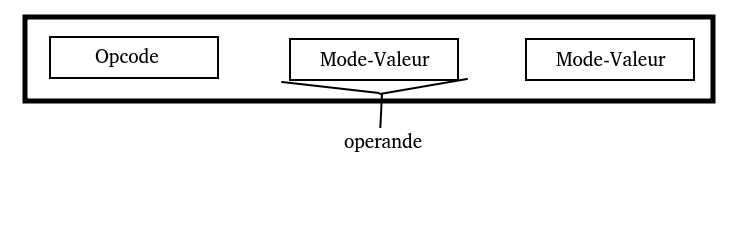
\includegraphics[scale=0.5]{Images/structure-operation.png}
	\caption{struture d'une operation}
\end{figure}

\begin{itemize}
	\item \textbf{Operande}:\\
	      Une operande est la combinaison d'un \textbf{mode d'addressage} et d'une valeur. Couramment la première opérande est dénommé l’\textbf{opérande A} et la seconde l’\textbf{opérande B}
	\item \textbf{Opcode}:\\
	      Les Opcodes sont utilisés pour spécifier quelles opérations devrait être réalisé quand une ligne de code est exécutée.\\
	      Fondamentalement on a huits(8) opcodes qui existent.\\
	      \begin{table}[h!]
		      \center
		      \begin{tabular}{|c|c|l}
			      \cline{1-2}
			      Opcode & Mnemonique & \\ \cline{1-2}
			      0      & DAT        & \\ \cline{1-2}
			      1      & MOV        & \\ \cline{1-2}
			      2      & ADD        & \\ \cline{1-2}
			      3      & SUB        & \\ \cline{1-2}
			      4      & JMP        & \\ \cline{1-2}
			      5      & JMZ        & \\ \cline{1-2}
			      6      & DJZ        & \\ \cline{1-2}
			      7      & CMP        & \\ \cline{1-2}
		      \end{tabular}
		      \caption{Listes des Opcodes}
	      \end{table}
	\item \textbf{Modes d'addressages}:\\
		Ainsi, les différentes modes d'addressages combinées aux valeurs pour former une opérande.
		Fondamentalement, on a quatre(4) modes d'addressage.
		\begin{table}[h!]
			\begin{tabular}{|l|l|}
			\hline
			Modes d'Addressage                       & Les octothorpes \\ \hline
			Mode d'addressage immediate              & \#              \\ \hline
			Mode d'addressage  direct                & \$ par défaut   \\ \hline
			Mode d'addressage indirect               & @               \\ \hline
			Mode d'addressage pre-decrement indirect & \textless{}     \\ \hline
			\end{tabular}
			\caption{Les modes d'addressage}
			\end{table}
			
\end{itemize}

\newpage

En effet, nous avons ci-dessous les huit(8) opérations de base et leur définitions ou leurs actions:

\begin{table}[h!]
	\center
	\begin{tabular}{|l|l|l|}
		\hline
		Opcode & Mnemonique & Définitions                                                   \\ \hline
		1      & DAT        & \begin{tabular}[c]{@{}l@{}}permet de retirer le processus en cours d'exécution \\ de la file d'attente des processus\end{tabular}                                     \\ \hline
		2      & MOV        & permet déplacer une opérande A vers une autre opérande B      \\ \hline
		3      & ADD        & permet d'ajouter une opérande A à une opérande B              \\ \hline
		4      & SUB        & permet de soustraire une opérande A d'une opérande B          \\ \hline
		5      & JMP        & permet de sauter à une opérande A                             \\ \hline
		6      & JMZ        & permet de sauter à une opérande A si une opérande B est nulle \\ \hline
		7      & DJZ        & \begin{tabular}[c]{@{}l@{}}permet de décrémenter l'opérande B; \\ si l'opérande B est nulle, on saute à l'opérande A\end{tabular}                                     \\ \hline
		8      & CMP        & \begin{tabular}[c]{@{}l@{}}permet de faire passer une instruction suivante si une opérande\\  A est égale à une opérande B\end{tabular}                                     \\ \hline
	\end{tabular}
	\caption{Listes et Définitions des Opcodes}
\end{table}

 

\subsection{Les différentes versions}
Il existe un certain nombre de versions du Redcode. La version la plus ancienne décrite par \textbf{\color{blue}Alexander Keewatin Dewdney} diffère à bien des égards des normes ultérieures établies par \textbf{l'International Core War Society}, et pourrait être considérée comme un langage différent, bien que connexe. La forme de Redcode la plus couramment utilisée aujourd'hui est basée sur un projet de norme soumis à l'ICWS \footnote{l'International Core War Society} en 1994, qui n'a jamais été officiellement accepté, l'ICWS ayant été dissoute à cette époque. Le développement de Redcode s'est cependant poursuivi de manière informelle, principalement via des forums en ligne tels que l'ICWS.\\

\underline{\textbf{\color{red}NB}}: Bien que durant ce projet nous avons cherché à se rapprocher des versions standards, il sera présenté une version un peu plus personnalisé.
\section{Analyse et Planification du projet}
Pour mener à bien le projet, il est nécessaire d'établir assez tôt le cahier des charges, l'architecture du projet et les objectifs qu'il faut atteindre en précisant les différentes deadlines.
\subsection{Les objectifs de conception}
Il est attendu à la fin du projet de livrer un outil permettant de générer des programmes efficace au CoreWar. De ce fait, il a fallu adapter nos différents objectifs pour aboutir au produit final qui est demandé.
\subsubsection*{Les objectifs principaux}
Ces objectifs se déclinent respectivement en 3 points par ordre de priorités:
\begin{itemize}
	\item \textbf{Développement d'une plateforme de simulation de la
		      machine virtuelle}
	\item \textbf{Exécution des programmes écrits en RedCode}
	\item \textbf{Implémentation d'un algorithme génétique}
\end{itemize}
Ainsi, ces trois(3) objectifs permettront d'aboutir au produit souhaité.
\subsubsection*{Les objectifs secondaires}
Il a été fixé principalement comme objectif secondaire, la réalisation d'une interface graphique qui faciliterait l'utilisation du programme.
\subsection{L'architecture du projet}
Les objectifs étant claires, il est nécessaire de bien structurer son projet. Il a été découpé au plusieurs packages qui nous permettent d'avoir une meilleur vue d'ensemble du projet.

\begin{figure}[h!]
	\center
	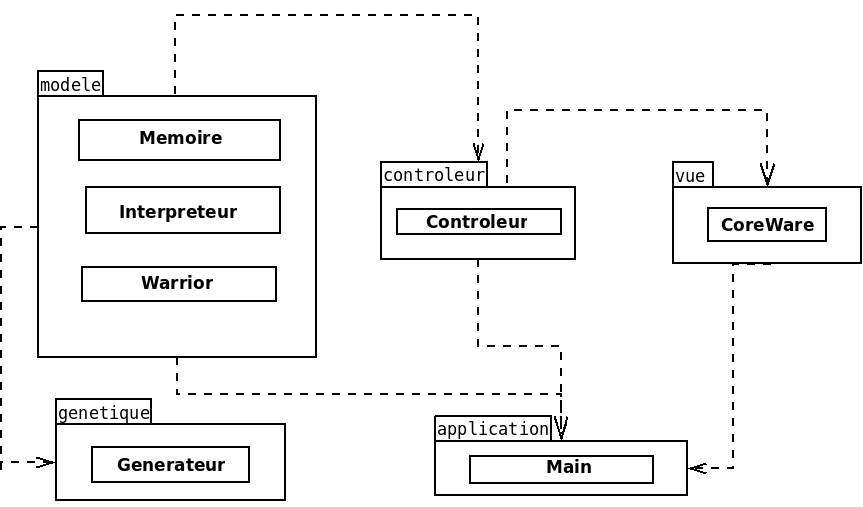
\includegraphics[scale=0.5]{Images/diagrammeDePackage.png}
	\caption{Diagramme de packages}
\end{figure}
Cela permet dès le début de voir les différents liens qu'il faudra établir et d'avancer plus sereinement dans le développement.
\subsection{Répartition des tâches}
Les tâches ont été réparti afin qu'à la fin du projet, il ne resterait plus qu'à combiner les différents codes de chacun. Etant dans un groupe de 3, il n'a pas été possible de s'organiser en binomes pour la réalisation du projet. De ce fait, il a fallu s'adapter. Un membre devrait s'occupait de la partie modèle du projet et un autre de la vue. Le troisième membre serait un électron libre qui devait passer d'une partie à l'autre par rapport à l'avancement du projet. Ainsi:
\begin{itemize}
	\item \textbf{Amirath} devrait se charger du début de l'implementation du modèle, précisement de la mémoire et des warriors
	\item \textbf{Sekou} commencerait ainsi les prémices de l'interface graphique
	\item \textbf{Emile} quant à lui implementerait de l'interpreteur des programmes de coreware, tout en apportant une main d'oeuvre dans les 2 autres parties que gérait Amirath et Sekou.Et par la suite s'occupera de la partie 
			génétique quand le projet serait à minima
\end{itemize}
\section{Conception du logiciel}
\subsection{Le choix du pattern}
Bien qu'ayant une vue assez globale du projet, le pattern \textbf{MVC}(\textbf{M}odèle \textbf{V}ue \textbf{C}ontroleur) a été choisi durant le projet. Ce choix était motivé par le fait que nous souhaitons que l'application finale permette une interaction avec l'utilisateur. Cela a permis ainsi de séparer la représentation des informations de notre modèle et la manière dont ces informations sont vues par l'utilisateur.
\subsection{Le modèle du jeu}
Pour le bon fonctionnement du modèle, il était nécessaire d'avoir au final trois(3) objets distincts:
\begin{itemize}
	\item \classname{memoire}
	\item \classname{Interpréteur}
	\item \classname{Warrior}
\end{itemize}
Ces trois(3) objets sont eux même constitués de sous objets qui permettre leur bon fonctionnement. Étant donnée qu'ils sont globalement indépendant, le choix a été fait de les développer dans des sous-packages du modèle(Voir Annexe).\\
\begin{figure}[h]
	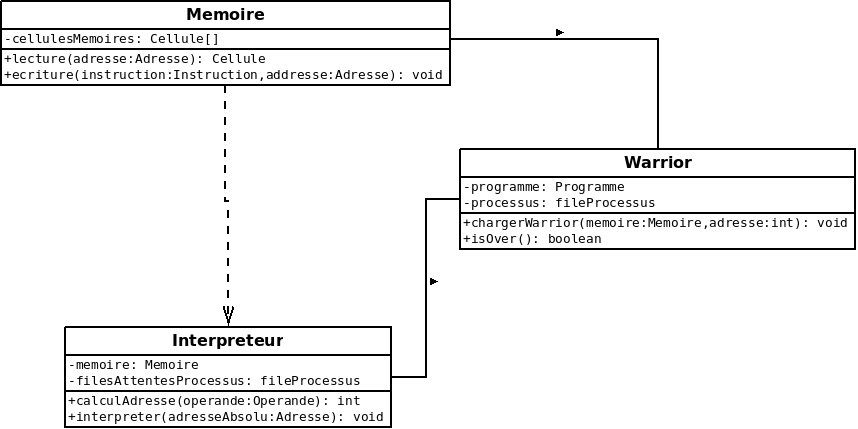
\includegraphics[scale=0.5]{Images/diagrammeModele.png}
	\caption{diagramme du modele de l'application}
\end{figure}
\subsubsection*{La mémoire}
C'est l'un des Objets les plus importants. Ce dernier permet de modélisé une mémoire virtuel pour notre MARS. Il est composé de cellules mémoire dans lesquels sont écrits les opérations de RedCode. Grace à cet objet, on a la possibilté de réaliser les operations de bases d'une machine à savoir:
\begin{itemize}
	\item \textbf{Lecture} à travers la méthode \methodname{lecture(Adresse adresse)}. On peut alors accéder à une cellule de la mémoire et voir son contenu.
	\item \textbf{Écriture} à travers la méthode \methodname{ecriture(Instruction instruction, Adresse adresse)}. On accède à la cellule situé à une adresse et on y écrit une nouvelle instruction
\end{itemize}

\subsubsection*{L’Interpréteur}
Comme son nom l'indique, il permet d'interpréter des instructions stockés dans la mémoire. Ainsi, pour son fonctionnement il a uniquement besoin de la mémoire sur laquelle il effectue l’interprétation et de l’adresse qu'il doit interpréter. On utilise principalement une seule méthode de la classe qui celle lié à l’interprétation d'une adresse: \methodname{interpreter}.
L'implementation de cet interpreteur permet d'analyser jusqu'à 10 types d'instructions distinctes
\subsubsection*{Le Warriror}
Les warriors sont les protagonistes de la bataille pour le controle de la mémoire. A travers cet objet, on peut principlaement maintenant:
\begin{itemize}
	\item Charger un warrior
	\item savoir l'état du warrior
\end{itemize}
\subsection{Le contrôle du jeu}
Pour cette application, le choix a été fait de centraliser le déroulement d'une partie dans un unique objet : \classname{Controleur}.
Cet objet gère totalement la mécanique de l'application. Il utilise principalement 2 objets du modèle :
\begin{itemize}
	\item Interpreteur
	\item Warrior
\end{itemize}
Ainsi, en utilisant un controleur, on gère le placement des warriros dans des zones mémoires séparées par une distance minimal.
La gestion des tours de jeu devient un peu plus naturel grâce à cette centralisation. On passe d'un tour à un autre en faisant
usage de la méthode \methodname{void excecute()}.

\begin{figure}[h]
	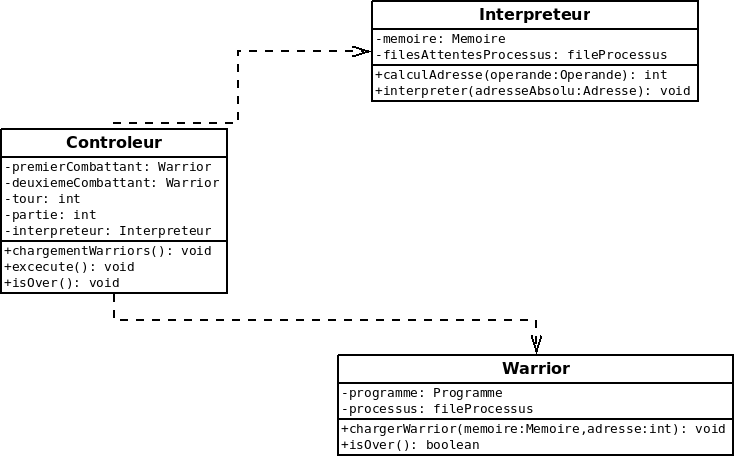
\includegraphics[scale=0.45]{Images/diagrammeControleur.png}
	\caption{Diagramme du package Controleur}
\end{figure}


\subsection{Interface Graphique}
Pour cette première version de l'application, le choix a été fait d'avoir une interface graphique qui
permettrait un usage facile pour l'utilisateur. En outre l'écran d'accueil, un écran principale a été développé
pour l'usage pratique de l'application. Ainsi l'utilisateur a la possibilité de naviguer d'un écran à l'autre, bien que La
plus grande partie de son interaction se résume à l'ecran de jeu.
\begin{figure}[h!]
	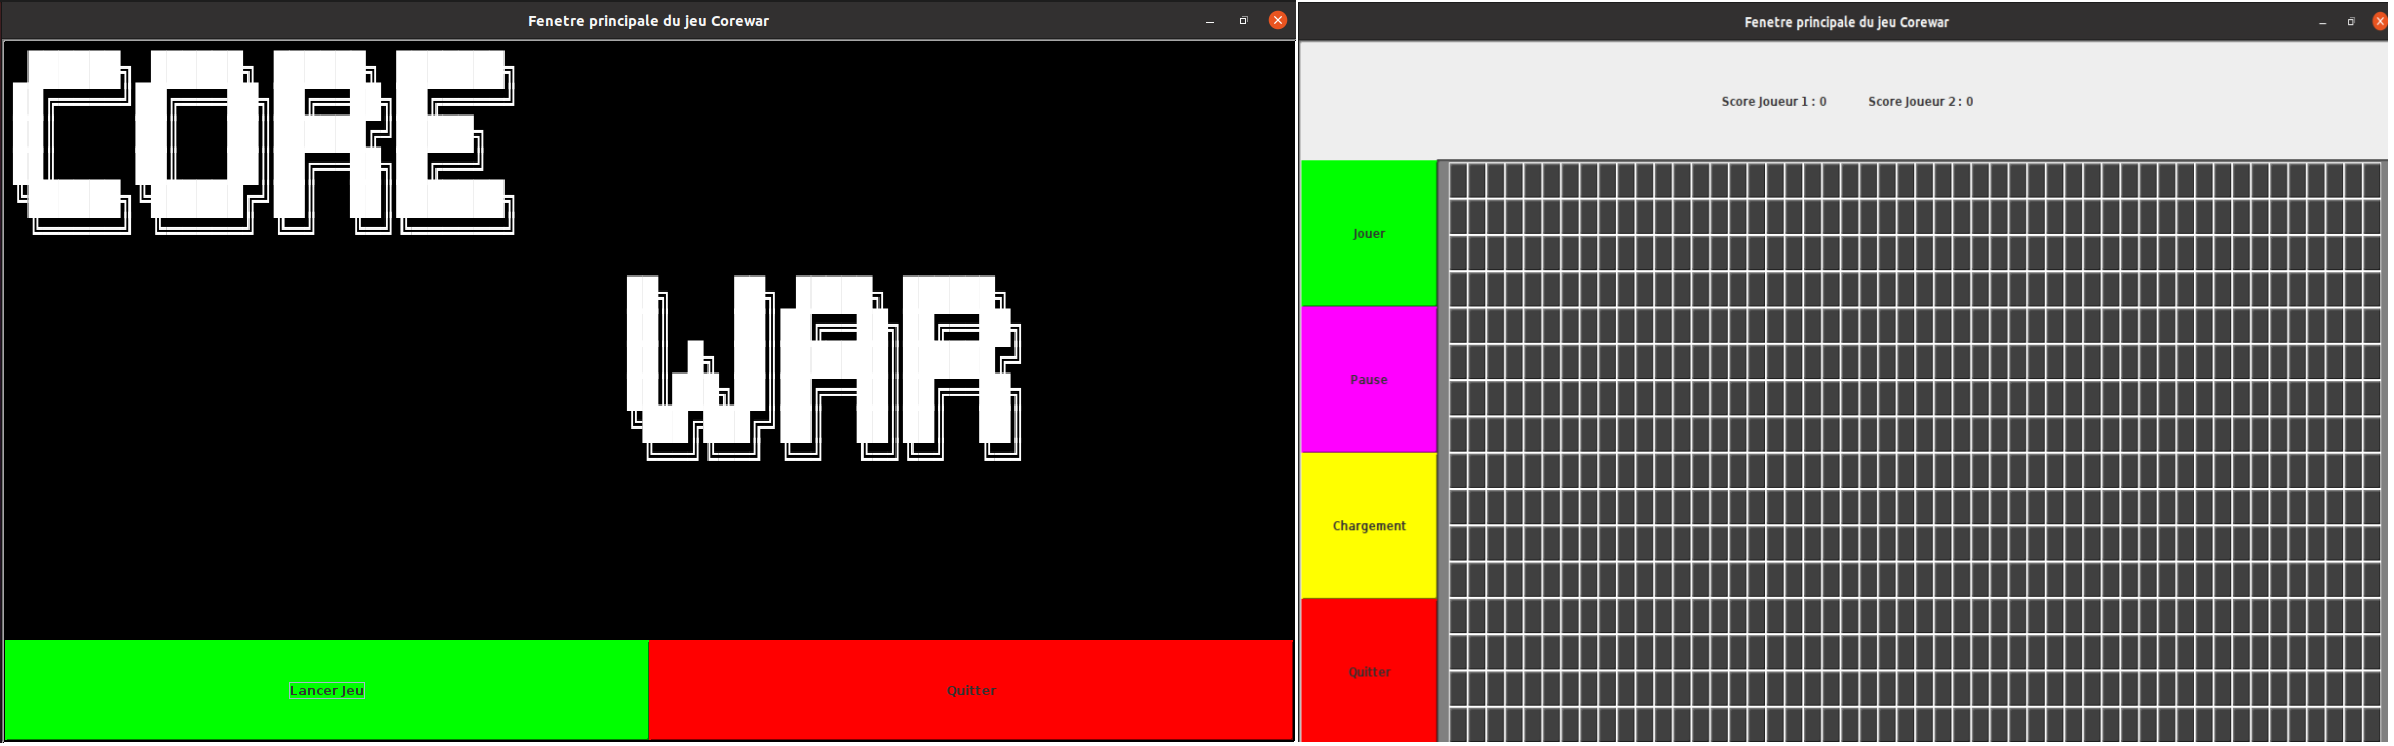
\includegraphics[scale = 0.27]{Images/ecransVue.png}
	\caption{Les écrans de la vue}
\end{figure}

Concernant l'écran de jeu, Il est décomposer en 3 grandes parties:

\begin{itemize}
	\item Une zone de boutons
	\item Une zone d'nformation où sont affiché le score de chaque joueur
	\item un plateau de jeu sur lequel se déroule le jeu
\end{itemize}

À travers notre interface graphique, nous avons la possibilité:
\begin{itemize}
	\item Charger le programme contenu dans les warriors dans la memoire
	\item Lancer un combat entre les 2 warriros
	\item Reinitialiser la partie(vider la memoire et la file d'attente des processus)
	\item Charger directement son propre programme de redCode dans l'un des warriros
	\item Mettre en pause une partie courante
\end{itemize}

\subsection{La génétique}
Pour modeliser notre système de génétique, il a fallu programmer les principes de bases d'une génétique
naturelle:
\begin{itemize}
	\item L'évaluation d'un individu de notre population c'est à dire un \classname{Programme}
	\item Effectuer les operations génétiques de bases(croisement et mutation)
	\item Comparer deux individus de la population
\end{itemize}
Les relations dans la \packagename{genetique} sont uniquement des relations d'associations
Aucune ne dépend d'une autre dans ce package. Tout est centraliser dans le générateur où nous
gérons les mutations et les croisements des programmes. Ainsi on utilise principalement les méthodes:
\begin{itemize}
	\item \methodname{croisementProgramme} de \classname{Croisement} pour retourner 2 fils issu du croisement de 2 parents
	\item \methodname{mutationProgramme} de \classname{Mutation} pour effectuer la mutation d'un programme en fonction des probabilité
		liées à sa réalisation
	\item \methodname{generate} de \classname{Generateur} pour générer un population futur à partir d'une population de base
	\item \methodname{generateProgramme}, elle utilise \methodname{generate} pour générer un programme efficace.S
\end{itemize}
\begin{figure}[h!]
	\center
	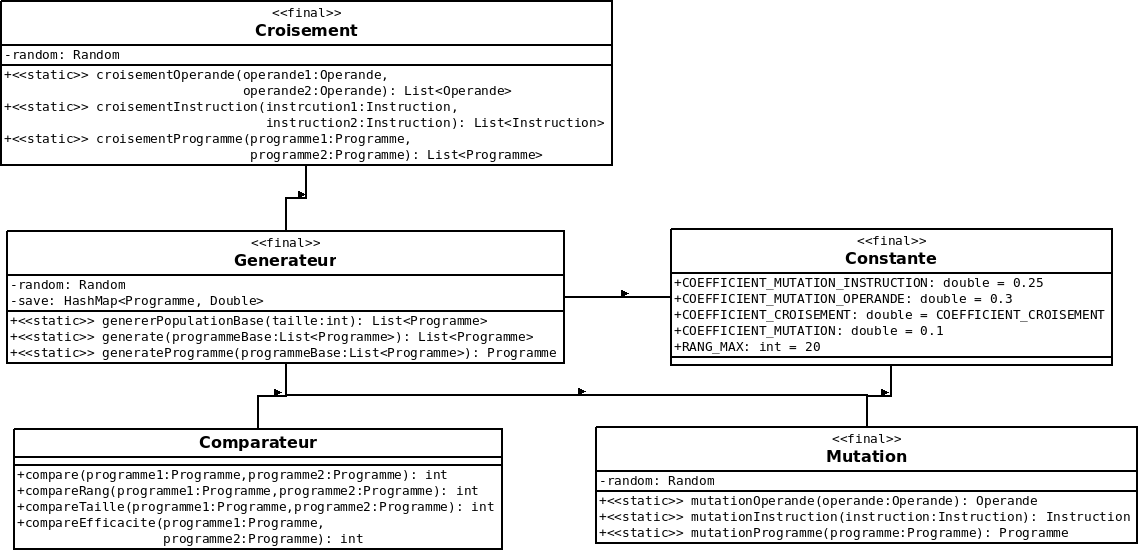
\includegraphics[scale = 0.45]{Images/diagrammeGenetique.png}
	\caption{diagramme du package génétique}
\end{figure}
\newpage
\section{Points techniques}
\subsection{Lecture et Interprétation des fichiers}
L'application permet de lire et interpréter les fichiers possédant du redCode. 
\subsubsection*{Le format de fichier}
Pour réaliser une lecture, le fichier doit répondre à une certaine norme prédéfinie:
\begin{itemize}
	\item Chaque ligne ne possédant pas du code doit débuter par le caractère '\textbf{\color{red};}'
	\item Une ligne de redCode ne doit contenir que les expressions en redCode et rien d'autres
	\item Le fichier ne peut pas contenir de ligne vide ni au début ni entre les lignes de code ou à la fin du fichier
	\item Une ligne de redCode doit obligatoirement être de la forme : opcode operande operande (par exemple MOV \$ 0 \$ 1)
\end{itemize}
\subsubsection*{Interprétation de fichier}
Si le fichier respecte le format prédéfini, l'interpretation de ce dit fichier lira chacune des lignes en les transformant en \classname{Instruction}
grâce à:
\definecolor{pblue}{rgb}{0.13,0.13,1}
\definecolor{pgreen}{rgb}{0,0.5,0}
\definecolor{pred}{rgb}{0.9,0,0}

\lstset{language=Java,
  commentstyle=\color{pgreen},
  keywordstyle=\color{pblue},
  stringstyle=\color{pred},
  basicstyle=\ttfamily,
  numbers=left,
  numberstyle=\tiny,
  frame=single,
  title=\lstname
}

\lstinputlisting[firstline=104, lastline=115, tabsize=3, framexleftmargin=-16pt,numbersep=-8pt,xleftmargin=-18pt]{../src/modele/redcode/instruction/Instruction.java}
\subsection{Logique de l'Interpréteur du MARS}
\subsubsection*{Retour sur le calcul d’adresse}
Pour le bon déroulement d'une partie, il est indispensable de bien effectuer les calculs d'adresses. Il se base sur le principe d'une mémoire
circulaire et l'utilisation des modes d'adressage pour pour calculer l'adresse effective.\\
La memoire circulaire est utile dans le sens où les operations n'aboutiront jamais à des zones mémoires non existantes. Ainsi 
pour chaque adresse on effectue son modulo \footnote{Le modulo est le reste de la division entiere d'un nombre a par un nombre b} avant de l'utiliser:\\
\[\boxed{adreseUtilise=addresseFourni \mod TAILLEMEMOIRE}\]
\subsubsection*{La gestion des processus}
Chaque Warrior possède un ou plusieurs processus. Lorsque le warrior est chargé pour la première fois dans le Core, 
il reçoit un seul processus, mais il peut en acquérir d'autres en exécutant l'instruction spl.\\

Pendant une partie de Corewar, chaque guerrier exécute à tour de rôle un seul processus. Dans le premier cycle du tour, 
le premier guerrier exécute une instruction. Dans le cycle suivant, le guerrier suivant exécute une instruction. 
Une fois que chaque guerrier a exécuté son tour, le premier guerrier recommence.\\

Si aucun guerrier n'exécute une instruction spl, c'est tout ce qu'il y a à faire et 
l'exécution continue de cette façon, chaque guerrier prenant son tour au cours des cycles successifs 
jusqu'à la fin du tour.\\

Lorsqu'une instruction spl est exécutée, le guerrier qui l'exécute gagne un nouveau processus. 
Maintenant, lorsque le guerrier prend son tour, il exécute un processus et lorsqu'il prend son 
tour suivant, il exécute l'autre processus.\\

Un exemple de gestion avec 2 warrior dont le premier warrior(en rouge) possede 2 processus et le second(en bleu)
un seul processus
\begin{figure}[h!]
	\center
	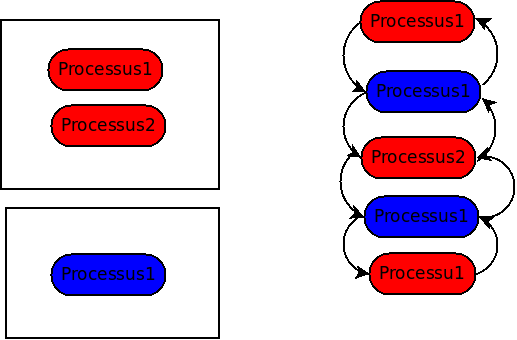
\includegraphics[scale=0.5]{Images/deroulementInterpreteur.png}
	\caption{Exemple de deroulement d'une partie}
\end{figure}
\subsection{Algorithm Génétique: Les principes de bases}
Un algorithme génétique (AG) est une métaheuristique inspirée par le processus de sélection naturelle qui appartient à la grande classe 
des algorithmes évolutionnaires (EA). Les algorithmes génétiques sont couramment utilisés pour générer des solutions de haute qualité à 
des problèmes d'optimisation et de recherche en s'appuyant sur des opérateurs d'inspiration biologique tels que la mutation, 
le croisement et la sélection.\\

Ce classe d'algorithm suit un certain ordre logique durant lesquels on effectue des operations bien précise
dans un ordre données:
\begin{itemize}
	\item Evaluation de la population initiale
	\item Selection des futures parents de la prochaine génération
	\item croisement et mutation de la population
\end{itemize}

\begin{figure}[h!]
	\center
	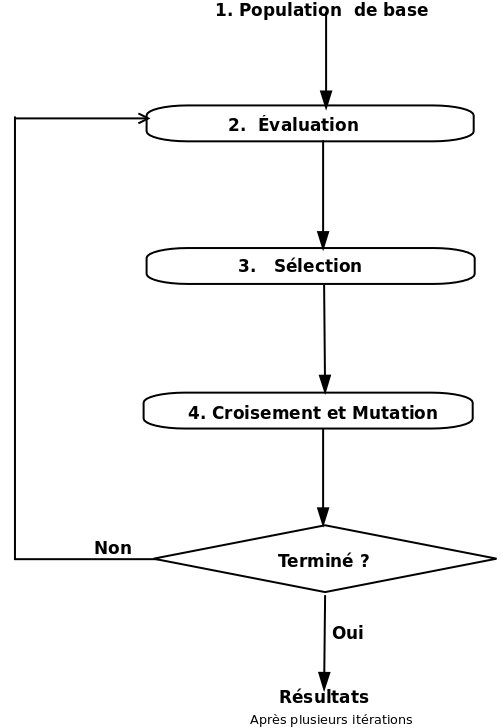
\includegraphics[scale=0.3]{Images/schema_recaputilatif_algorithm_genetique.png}
	\caption{Shéma recaputilatif d'un algorithm génétique}
\end{figure}

\newpage
Ainsi notre algorithm est basé sur des mutations et des croisements probabilistes:

\begin{itemize}
	\item La mutation des operandes est réalisé que dans 30\% des cas
	\item La mutation des opcodes est effectué dans 25\% d'une population
	\item La mutation des instructions se déroule dans 10\% des cas
	\item Le croisement entre 2 parents donnent des enfants dans 70\% des croisements
\end{itemize}

Pour aboutir à un programme efficace, on passe par 2 algorithm distincts:\\
Le premier algorithm nous montre comment aboutir à un programmme efficace
\begin{algorithm}[h!]
	\DontPrintSemicolon
	\SetKwData{PopulationBase}{populationBase}
	\SetKwData{ProgrammeEfficace}{ProgrammeEfficace}
	\KwIn{Une collection de programmes $\PopulationBase=\{p_1, p_2, \dots, p_n\}$ où chaque programme est une liste d'instructions
			ecrits en redCode}
	\KwOut{Un programme efficace}
	\uIf{$Taille(PopulationBase) == 1$}{
		$\ProgrammeEfficace \gets p_1$\;
		\uIf{$efficacite(\ProgrammeEfficace) > 0.8$}{
			\Return{$\ProgrammeEfficace$}\;
		}
		$\PopulationBase \gets \PopulationBase \cup \{copie(p_1)\}$\;
	}
	\Return{$generationFutur(populationBase)$}\;
	\caption{Générer un programme efficace}
\end{algorithm}

Le second explique comment s'effectue la génération d'une futur population
\newpage
\begin{algorithm}[h!]
	\DontPrintSemicolon
	\SetKwData{PopulationBase}{populationBase}
	\SetKwData{FutureGeneration}{futureGeneration}
	\KwIn{Une collection de programmes $\PopulationBase=\{p_1, p_2, \dots, p_n\}$ où chaque programme est une liste d'instructions
			ecrits en redCode}
	\KwOut{Une future génération composée des parents de la populations de bases et de leurs enfants aynt subi une mutation ou pas}
	$\FutureGeneration \gets \emptyset$\;
	$parents \gets \emptyset$\;
	\While{$Taille(parents) < Taille(\PopulationBase) / 2 $ }{
		$programme \gets $un programme aléatoire dans $\PopulationBase$\;
		$efficaciteMin \gets \gets$ un réel entre 0 et 1\;
		\uIf{$efficaciteMin < efficacite(programme)$ ou $ efficaciteMin > 0.7$}{
			$parents \gets parents \cup \{programme\}$\;
		}
	}
	$\FutureGeneration \gets \FutureGeneration \cup \{parents\}$\;

	\While{$parents \neq \emptyset $}{
		$parent1 \gets aléatoirement un élément de parents$\;
		$parent2 \gets aléatoirement un élément de parents$\;
		$probabilite \gets$ un réel entre 0 et 1\;
		\uIf{$probabilite > PROBABILITECROISEMENT$}{
			$\FutureGeneration \gets \FutureGeneration \cup \{croisement(p1, p2)\}$\;
		}
		$parents \gets parents - \{p1, p2\}$\;
	}

	\ForEach{Programme p dans $\FutureGeneration$}{
		$probabilite \gets$ un réel entre 0 et 1\;
		\uIf{$probabilite > PROBABILITEMUTATION$}{
			$\FutureGeneration \gets \FutureGeneration \cup {mutation(p)}$\;
			$\FutureGeneration \gets \FutureGeneration - {p}$\;
		}
	}
	\Return{$\FutureGeneration$}\;
	\caption{Generation d'une population à partir d'une autre population}
\end{algorithm}

Ainsi grace à la combinaison des 2 algorithmes, nous trouvons une solution à notre problème
d'optimisation
\section{Expérimentations sur l'algorithm Génétique}
Le but principale de ces expérimentations été de montrer que le caractère aléatoire de la génétique sont respecté et également de montrer la convergence vers un programme efficace.
\subsection*{Conditions d'Expérimentations}
Afin de pouvoir fournir des conclusions logiques, certains choix ont été
fait pour ne pas biaisés les conclusions et les résultats obtenus :

\begin{itemize}
	\item Pour chaque données utilisés est la moyenne des résultats répétées ayant une même taille de la population de base
	\item Pour chaque expérience doit être faite à partir de graines différentes pour l'aléatoire
	\item Le critère fondamentale de ces expérimentation est lié à la taille de la population d'entrée
\end{itemize}

\subsection*{Analyse et interprétation des résultats}
\begin{figure}[h!]
	\begin{center}
		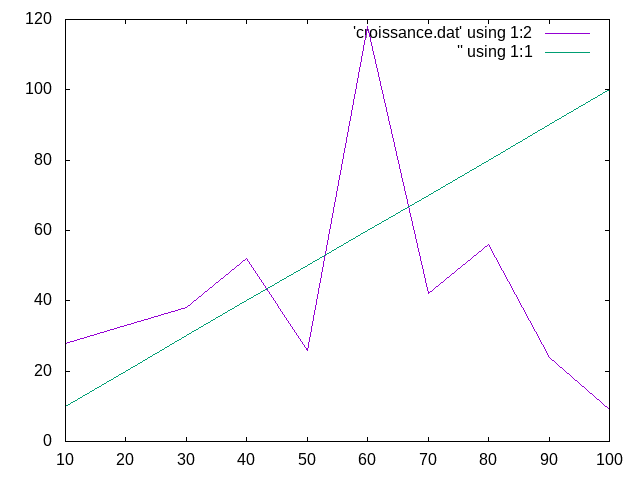
\includegraphics[scale=0.4]{Images/croissance.png}
	\end{center}
	\caption{Courbe du nombre de tour effectué en fonction de la taille de la population}
\end{figure}
La figure obtenue ne permete pas d'établir à premiere vue que la recherche d'un programme efficace soit liés à la taille des 
données mises en entrée. On obtient une courbe en zig-zag qui est loin de suivre l'allure d'une fonction
mathématique classique ou connus.Ainsi nous ne pouvons comparer la courbe pour estimer une convergence. Toutefois on remarque qu'il est assez rare 
de dépaser 60 tour pour obtenir un efficace.\\
\begin{figure}[h!]
	\begin{center}
		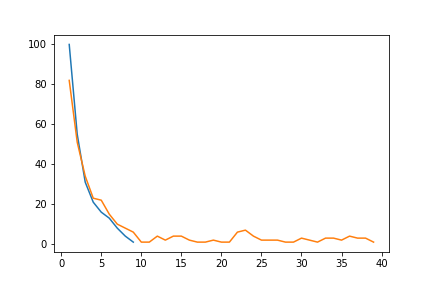
\includegraphics[scale=0.5]{Images/decroissancePopulation.png}
	\end{center}
\end{figure}
Cette figure montre la variation de la population de base. C'est à dire elle fait apparait la taille de la population
durant la recherhce d'un programme efficace. Cette courbe est à une allure decroissant dans sa majeur partie.
Il existe néamoins des zones où la population croit avant de décroite de nouveaux.
\subsection*{Conclusion}
En somme, l'allure en zig-zag du nombre de tour effectué avant l'aboutissant à un programme éfficace
permet de conclure que l'algorithm génétique respecte bien les lois de la génétique qui pronent le fait que 
l'aboutissement à un individu ayant de bonne caractéristique n'est pas lié en soit à la taille de la population initiale
mais à la faculté d'adaptation de ces individus à leur environnement. De plus l'évolution de la population durant la 
recherche d'un individu idéale est assez variable. Toutefois vu le caractère elitisme de tout notre algorithm,
on assiste à une décroissance rapide de cette population qui ne garde que ses meilleurs individus pour être les parents 
de la future génération et donc ameliorer leur capacité d'adaptation.\\

Il en revient en dernier lieu, qu'il n'est pas evident d'étudié le comportement d'un algorithm génétique. Cela
est dû notamment au fait que l'algorithm se base sur des principes de selection naturelle et des variables probabilistes.
Cependant nous pouvons néamoins remarquer le caractère elitisme de notre sélection qui permet d'aboutir rapidement
à un individu idéale.
\section{État d'avancement du projet}
\subsection{Un point sur les objectifs}
À ce jour, l'application remplit l'ensemble des objectifs fixés. Elle possède notamment:
\begin{itemize}
	\item Une machine virtuel fonctionnel. Cette machine virtuel possède une mémoire et un interpréteur permettant d'analyser 12 instructions
	\item Une implémentation de warrior qui permet de définir un combattant du jeu
	\item Une interface graphique qui permet d'avoir une visualisation globale du fonctionnement du coreware
	\item Un système de chargement de programme écrit en RedCode
	\item Un algorithm génétique qui fournit des warriors à partir d'une population d'entrée
\end{itemize}
\subsection{Les difficultés rencontrés}
Comme tout projet, il arrive de se retrouver dans des impasses. Cependant la grande partie d'entre eux ont été résolu après des remises en questions sur les choix faits(choix des structures de données, objets à créer, algorithm écrits ..). Cependant certaines ont été plus complexes que d'autres et reste jusqu'à cet stade sans une solution de notre part:
\begin{itemize}
	\item La gestion des processus multiples
	\item la recette idéale pour notre algorithm génétique
\end{itemize}
\subsection{Les améliorations possibles}
Bien que l'ensemble de l'application rentre dans le format attendu, il est possible de faire plusieurs ameliorations.
Parmis celle ci se trouve notamment:
\begin{itemize}
	\item \textbf{Amelioration de la version implémenté}:\\
		En effet, la version fournie nécessite une certaine modification des programmes en redCode récupéré en ligne. Ainsi dans de prochaine mise
		à jour, il serait important de corriger ce problème pour que l'utilisateur n'est plus à devoir réécrire les programmes dont il peut télécharger.
	
	\item \textbf{Implementer une version plus récent de redCode}:\\
		La version qui a été fourni se rapproche de la version ICW88 sans l'atteindre. Ainsi une première étape serait d'obtenir une application
		possédant cette version de redCode avant de passer aux versions plus récente.
	
	\item \textbf{Ameliorer l'interface graphique}:\\
		L'interface graphique fourni actuellement possède globalement les mêmes fonctionnalités que celle des versions fournis en ligne.
		Toutefois, on peut l'ameliorer notamment sur la representation cases memoires où un processus meurt. Ou fournir directement dans l'application
		une interface où l'utilisateur pourra écrire directement le code de ses warriors avant de les charger et les faire combattre sur le MARS
\end{itemize}
\section{Conclusion}
Dans ce projet nous nous fixés de réaliser une application qui interpreterait le langage de programmation \textbf{redCode} et ainsi nous permettre de pouvoir
mettre en concurrence 2 programmes pour le controle du MARS. De plus l'un de nos critères fondamentales fut la réalisation de l'interface
graphique. Pour ce faire, nous avons structurer notre application en utilisant un pattern MVC qui permettrait l'implementation d'une interface graphique. Nous avons
fait le choix de structurer notre modèle en différent package:
\begin{itemize}
	\item \packagename{redCode}
	\item \packagename{memoire}
	\item \packagename{combattant}
\end{itemize}
Ces packages du modèle nous ont permis de pouvoir modeliser une machine virtuel mais aussi de mettre en oeuvre le deroulement d'un partie
de coreware. Cela a été possible en combinant le module \packagename{redCode} avec \packagename{memoire} et \packagename{combattant}. Le controle du jeu
est quant à lui possible grâce à l'utilisation de l'ensemble du package \packagename{modele} et une gestion de tour de vue. Et la pierre angulaire du 
de l'application qui est la vue se résumait dès lors juste à une implementation des actions et une modelisation de la representation du modèle.\\

Pour conclure notre application nous avons proposé un algorithm génétique qui permet de générer un combat efficace. L'efficacité de ce combat est sa
faculté à pouvoir effectuer plusieurs tours de jeu sans auto détruire.

En somme, ce projet nous a permis d'ameliorer nos techniques de programmations, ameliorer la gestion des projets en groupe qui peut être fastidieuse.
Cela a permis également d'avoir une meilleur vision du coeur d'une machine et le déroulement de ses instructions.

\newpage

\nocite{*}
\bibliographystyle{abbrv}%ou plain, abbrv, alpha, apalike, ...
\bibliography{Bibliographie}

\newpage
\section*{Annexe}
\subsection*{Diagramme complet modele}
Cette section contient une vue plus globales du modèle en présentant les methodes principales
utilisés

\begin{figure}[h!]
	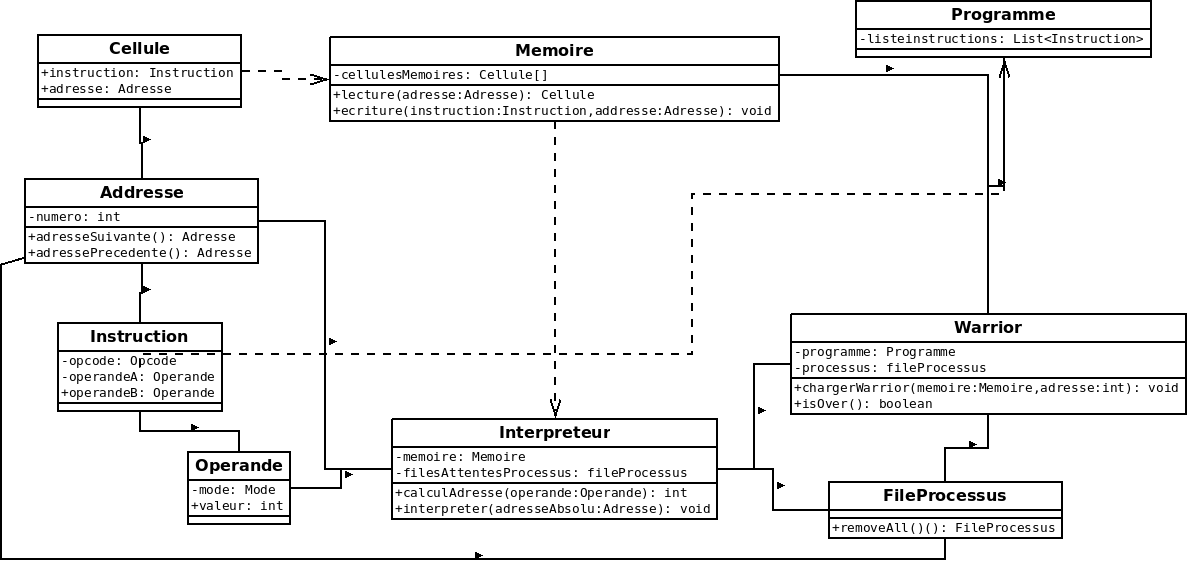
\includegraphics[scale=0.4]{Images/diagrammeModeleComplet.png}
\end{figure}
\end{document}
